%% Ein einfaches Template für einen Übungsbericht unter Verwendung des Hagenberg
%% Setups, basierend auf der LaTeX 'report' Standardklasse.
%%% äöüÄÖÜß  <-- keine deutschen Umlaute hier? UTF-faehigen Editor verwenden!

%%% Magic Comments zum Setzen der korrekten Parameter in kompatiblen IDEs
% !TeX encoding = utf8
% !TeX program = pdflatex
% !TeX spellcheck = de_DE
% !BIB program = biber

\documentclass[german,notitlepage,smartquotes]{hgbreport}
% Zulässige Optionen in [..]:
%    Hauptsprache: 'german' (default), 'english'
%    Option zur Umwandlung in typografische Anführungszeichen: 'smartquotes'
%    APA Zitierstil: 'apa'
%    Erzeuge keine separate Titelseite: 'notitlepage'
%%%-----------------------------------------------------------------------------

\RequirePackage[utf8]{inputenc} % bei Verw. von lualatex oder xelatex entfernen!

\renewcommand{\chapter}[1]{} % Deaktiviere den \chapter Befehl
\graphicspath{{images/}}     % Verzeichnis mit Bildern und Grafiken
\bibliography{references}    % Biblatex-Literaturdatei (references.bib)
\ExecuteBibliographyOptions{backref=false} % Keine Rückreferenzen bei Quellen

%%%-----------------------------------------------------------------------------
\setcounter{chapter}{3}	% <----- Auf die Übungsnummer setzen
%%%-----------------------------------------------------------------------------

\author{Julian Jany}                        % Name
\title{BVA2 Fortgeschrittene Bildverarbeitung und -analyse -- SS 2022\\ % Name der Übung
				Übungsabgabe \arabic{chapter}}
\date{\today}

%%%-----------------------------------------------------------------------------
\begin{document}
%%%-----------------------------------------------------------------------------
\maketitle
%%%-----------------------------------------------------------------------------

%\begin{abstract}\noindent
%\ldots
%\end{abstract}

%%%-----------------------------------------------------------------------------

\section{Richardson Lucy Deconvolution}

\subsection{Problembeschreibung}

Es soll ein \texttt{ImageJ Plugin} entwickelt werden. 
Das Plugin soll den iterativen Algorithmus \textit{Richardson Lucy Deconvolution} anwenden, und damit ein \zB unscharfes Bild "scharfstellen" können. 

\subsection{Lösungsbeschreibung}

\subsection{Implementierung}

Hier werden interessante Code-Teile der Implementierung inkludiert.

\subsubsection{Extraktion der Buchstaben}

\subsection{Tests}

\begin{figure}[h]
\centering
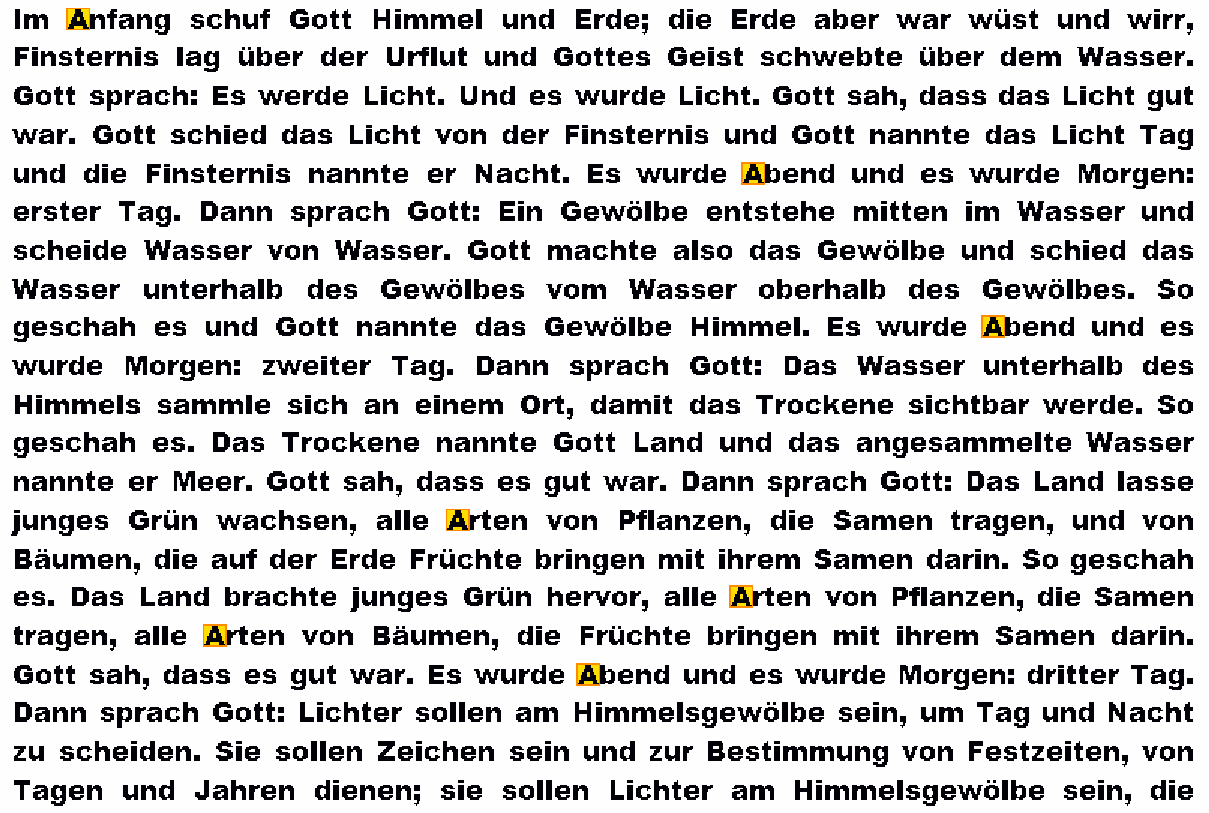
\includegraphics[width=.7\textwidth]{test-01-A}
\caption{Alle 'A' im Bild markiert.}
\label{fig:test-01}
\end{figure}

\begin{figure}[h]
    \centering\small
    \begin{tabular}{cc}
        \FramePic{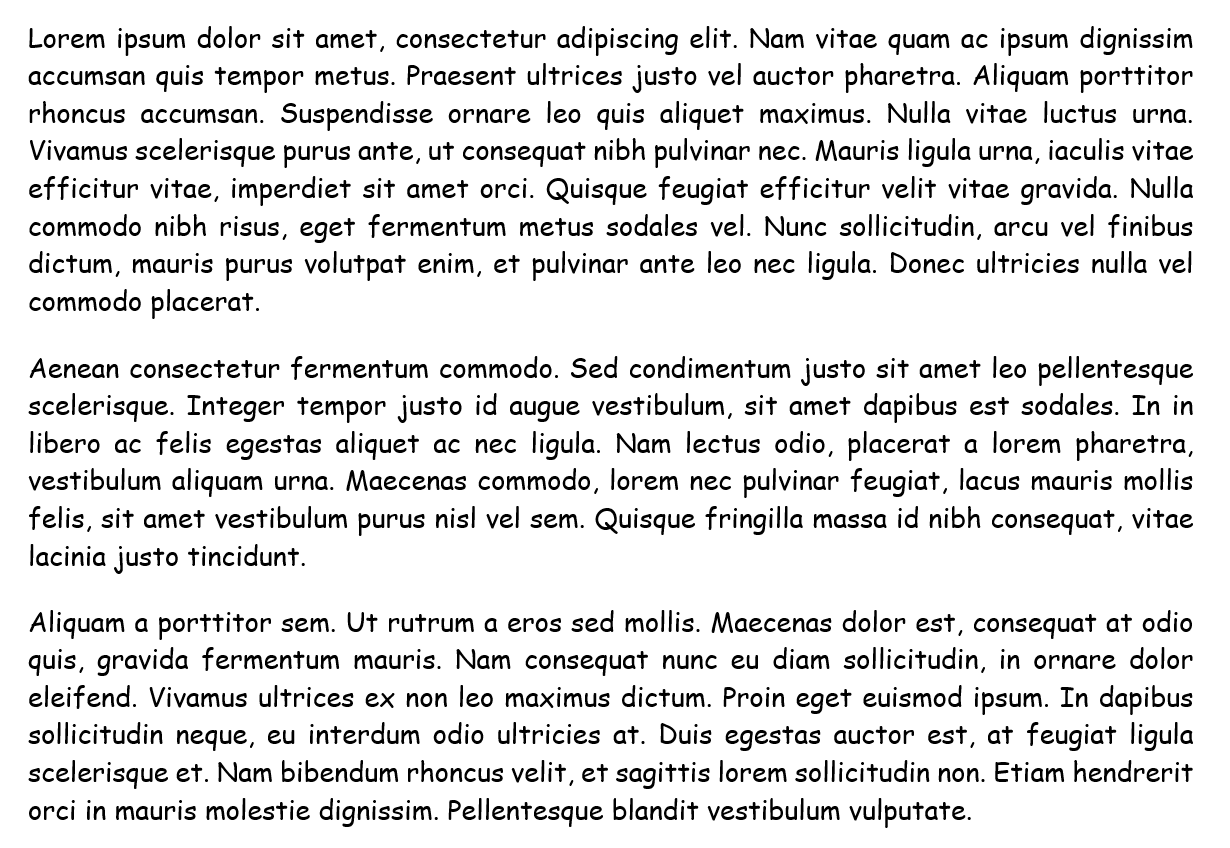
\includegraphics[width=0.5\textwidth]{comic_sans}} &
        \FramePic{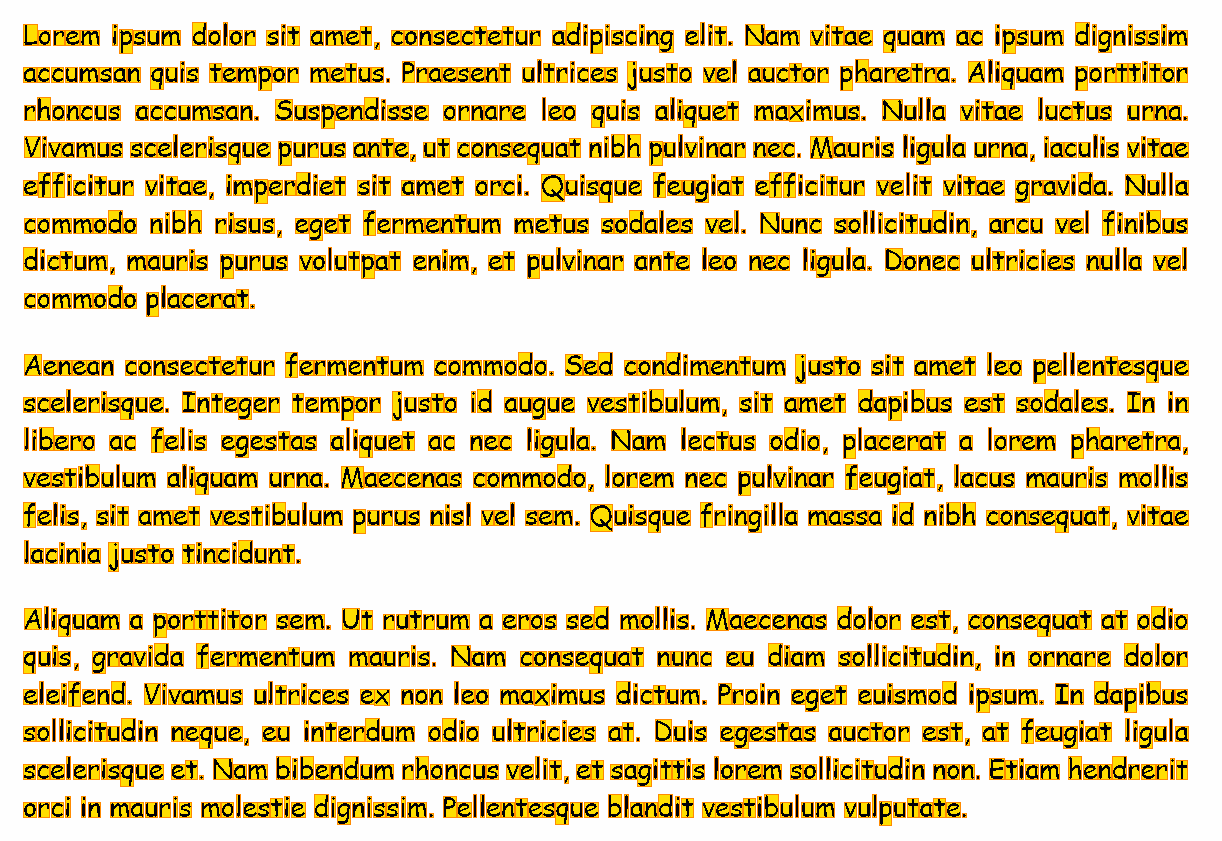
\includegraphics[width=0.5\textwidth]{test-09-comic_mark}} \\
        (a) & (b) \\
		\FramePic{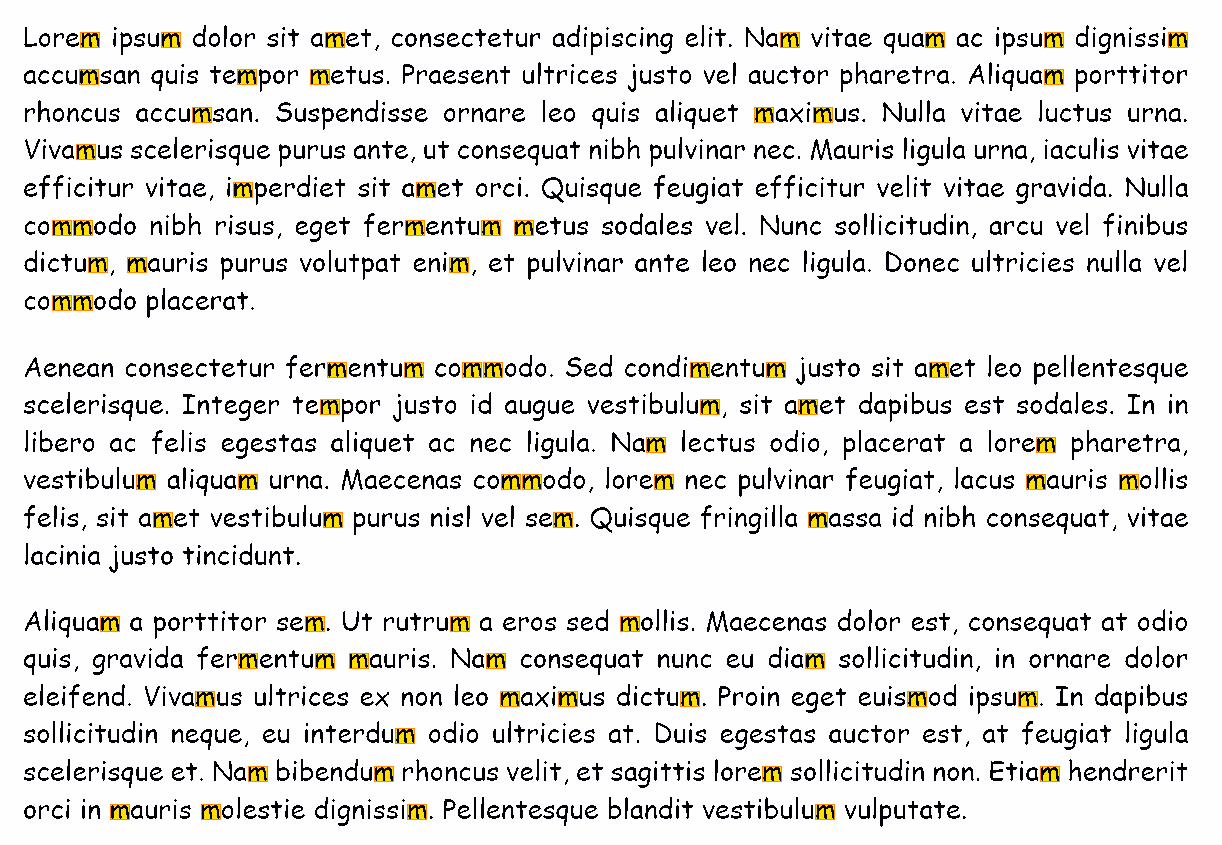
\includegraphics[width=0.5\textwidth]{test-09-comic-m}} &
        \FramePic{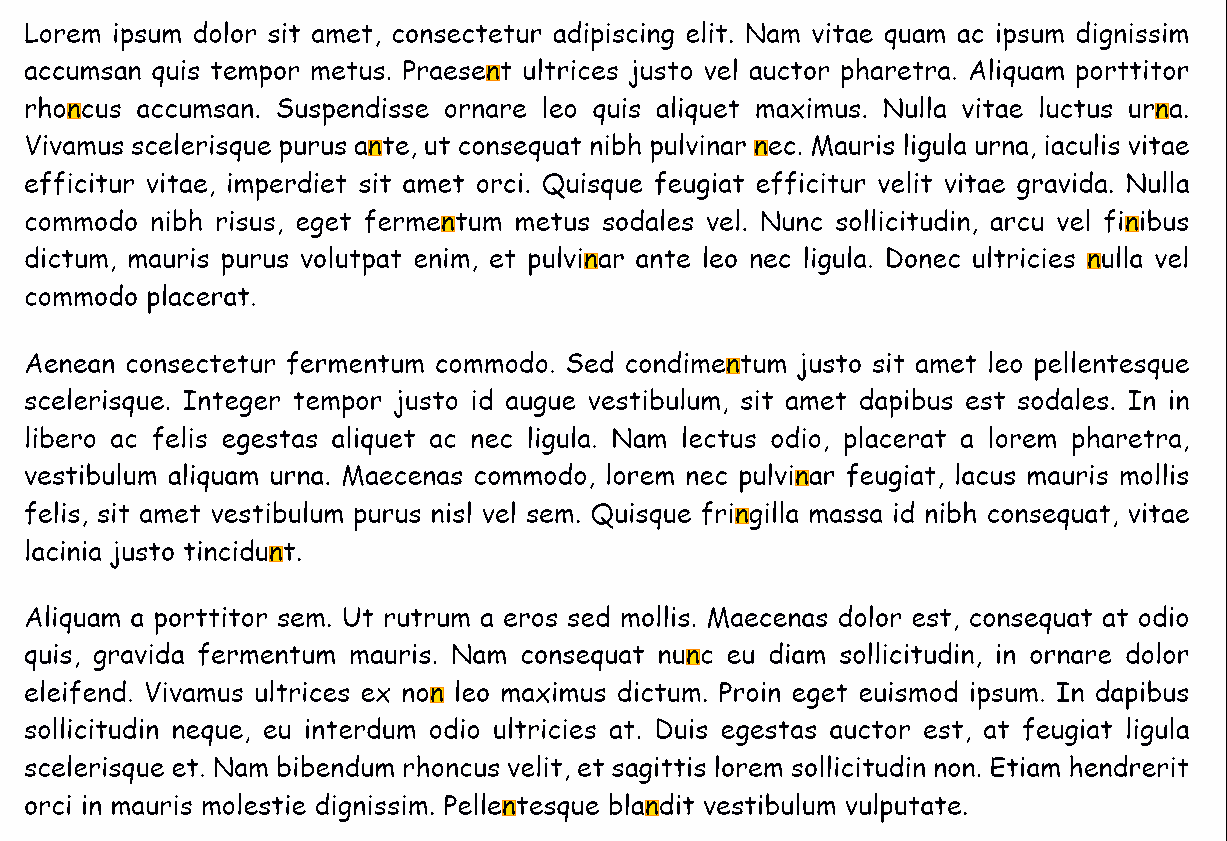
\includegraphics[width=0.5\textwidth]{test-09-comic-n}} \\
		(c) & (d)
    \end{tabular}
    \caption{Eingabe-Bild~(a); Extrahierte Buchtaben~(b); Alle 'm' markiert~(c) sowie alle 'n' markiert~(d).}
    \label{fig:test-09}
\end{figure}

\subsection{Diskussion}

%%%-----------------------------------------------------------------------------

% \section{Titel der zweiten Aufgabe}

%%%-----------------------------------------------------------------------------

%\section*{Zusammenfassung und Anmerkungen}

%%%-----------------------------------------------------------------------------

% \section*{Quellen}

% \printbibliography[heading=noheader]

%%%-----------------------------------------------------------------------------
\end{document}
%%%-----------------------------------------------------------------------------